\documentclass[tikz,border=3pt]{standalone}
\usepackage[utf8]{inputenc}
\usepackage[T1]{fontenc}
\usepackage{libertinus}
\usepackage{amsmath,amssymb}
\usetikzlibrary{arrows.meta,calc,patterns,decorations.pathmorphing,decorations.markings,decorations.pathreplacing,bending}
\definecolor{UGblue}{RGB}{0,51,102}
\newcommand{\dbar}{\mathchar'26\mkern-12mu d}
\tikzset{
  >=Stealth,
  every node/.style={font=\small},
  caja/.style={draw,line width=0.9pt},
  pared/.style={draw,line width=1.6pt},
  ejes/.style={->,line width=0.8pt},
  adia/.style={draw,pattern=north east lines,pattern color=black!70,line width=0.5pt},
  gas/.style={fill=UGblue!8},
  punto/.style={fill,circle,inner sep=1.3pt},
  onda/.style={decorate,decoration={snake,amplitude=1.1pt,segment length=5pt,post length=3pt,pre length=0pt}},
}
\begin{document}
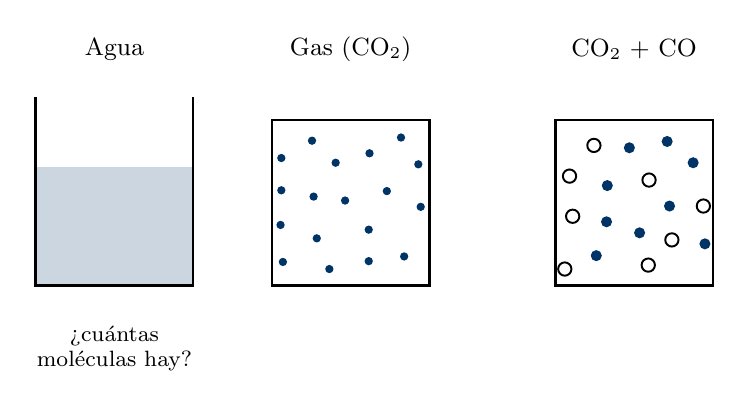
\begin{tikzpicture}
  % agua
  \fill[UGblue!20] (0,0) rectangle (2.0,1.5);
  \draw[caja] (0,2.4) -- (0,0) -- (2.0,0) -- (2.0,2.4);
  \node at (1.0,3.0) {Agua};
  \node[align=center] at (1.0,-0.8) {\footnotesize ¿cuántas\\[-2pt]\footnotesize moléculas hay?};
  % gas
  \draw[caja] (3,0) rectangle (5,2.1);
  \fill[UGblue] (3.53,1.13) circle (1.5pt);
  \fill[UGblue] (4.23,0.31) circle (1.5pt);
  \fill[UGblue] (3.12,1.62) circle (1.5pt);
  \fill[UGblue] (3.57,0.60) circle (1.5pt);
  \fill[UGblue] (4.89,1.00) circle (1.5pt);
  \fill[UGblue] (4.24,1.68) circle (1.5pt);
  \fill[UGblue] (4.46,1.20) circle (1.5pt);
  \fill[UGblue] (3.81,1.56) circle (1.5pt);
  \fill[UGblue] (4.68,0.37) circle (1.5pt);
  \fill[UGblue] (4.23,0.71) circle (1.5pt);
  \fill[UGblue] (4.64,1.88) circle (1.5pt);
  \fill[UGblue] (3.93,1.08) circle (1.5pt);
  \fill[UGblue] (3.14,0.30) circle (1.5pt);
  \fill[UGblue] (3.11,0.77) circle (1.5pt);
  \fill[UGblue] (3.51,1.84) circle (1.5pt);
  \fill[UGblue] (4.86,1.54) circle (1.5pt);
  \fill[UGblue] (3.73,0.21) circle (1.5pt);
  \fill[UGblue] (3.12,1.21) circle (1.5pt);
  \node at (4.0,3.0) {Gas (CO$_2$)};
  % mezcla
  \draw[caja] (6.6,0) rectangle (8.6,2.1);
  \fill[UGblue] (7.12,0.38) circle (2pt);
  \draw[line width=0.7pt] (6.82,0.88) circle (2.4pt);
  \fill[UGblue] (8.35,1.56) circle (2pt);
  \draw[line width=0.7pt] (8.08,0.58) circle (2.4pt);
  \fill[UGblue] (7.67,0.67) circle (2pt);
  \draw[line width=0.7pt] (7.09,1.78) circle (2.4pt);
  \fill[UGblue] (7.26,1.27) circle (2pt);
  \draw[line width=0.7pt] (7.79,1.34) circle (2.4pt);
  \fill[UGblue] (8.50,0.53) circle (2pt);
  \draw[line width=0.7pt] (6.78,1.39) circle (2.4pt);
  \fill[UGblue] (8.02,1.83) circle (2pt);
  \draw[line width=0.7pt] (8.48,1.01) circle (2.4pt);
  \fill[UGblue] (7.54,1.75) circle (2pt);
  \draw[line width=0.7pt] (7.78,0.26) circle (2.4pt);
  \fill[UGblue] (7.25,0.81) circle (2pt);
  \draw[line width=0.7pt] (6.72,0.21) circle (2.4pt);
  \fill[UGblue] (8.05,1.01) circle (2pt);
  \node at (7.6,3.0) {CO$_2$ + CO};
\end{tikzpicture}
\end{document}
